\section{ Theoretical Foundations}
\title[Theoretical Foundations]{Theoretical Foundations}

\begin{frame}{{Theoretical Foundations}}
     \begin{columns}
 	    \column{0.5\textwidth}
            \textbf{Information Theory}
            \begin{itemize}
                \item Entropy
                \item Kullback-Leibler Divergence
                \item Mutual Information
                \item Transfer Entropy
            \end{itemize}

 	    \column{0.5\textwidth}
            \textbf{Bayesian Networks}
            \begin{itemize}
                \item Bayesian Networks - Concept
                \item Structural Learning in Bayesian Networks
                \item K2-Algorithm
                \item Medium Description Length (MDL)
            \end{itemize}
	\end{columns}



\end{frame}

\begin{frame}{{Theoretical Foundations}}

% 	\begin{columns}
% 	    \column{0.5\textwidth}\centering
	       
	        
% 	    \column{0.5\textwidth}\centering
	      
% 	\end{columns}


\begin{align*}
   \centering \textbf{Entropy}
\end{align*}

Definition: The amount of information produced by an information source.

\begin{equation}
\label{eq:shannon}
    H = \sum_{i}^{n} p_{i}(i)log_{2}\frac{1}{p(i)}
\end{equation}

Properties: 
\begin{itemize}
    \item It is continuous in the domain of $p_i$, which is the probability mass function.
    \item It is monotonically increasing, in the \textit{n} domain, when all events are likely equally.
    \item It is weighted additive when a choice is broken down into successive choices. 
\end{itemize}
\end{frame}

\begin{frame}{{Theoretical Foundations}}

It is related to the frequency of the appearance of each value or the amount of surprise obtained given the appearance of a state or value.

\begin{figure}
    \centering
    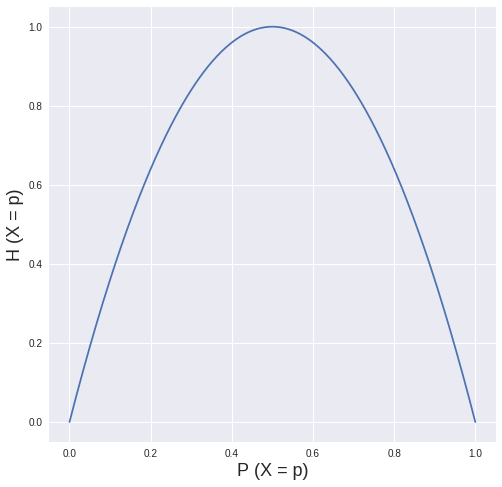
\includegraphics[scale=0.3]{figuras/entropy.png}
    \caption{Caption}
    \label{fig:my_label}
\end{figure}
\end{frame}

\begin{frame}[allowframebreaks]{{Theoretical Foundations}}

\begin{align*}
   \centering \textbf{Kullback-Leibler Divergence}
\end{align*}

\begin{itemize}
    \item Given  a variable I, with probability distribution \textit{p}. It measures the error or divergence when it is assumed that the probability distribution of I is \textit{q}, instead of \textit{p}.
\end{itemize}

\begin{equation}
\label{eq:kullback}   
    KL_{I} = \sum_{i}^{n}p(i)log \frac{p(i)}{q(i)}
\end{equation}

\begin{equation}
\label{eq:kullback_joint}   
    K_{I, J} = \sum_{i,j}^{n}p(i,j)log \frac{p(i,j)}{q(i,j)}
\end{equation}


\begin{equation}
\label{eq:kullback_cond}   
    K_{I \mid J} = \sum_{i,j}^{n}p(i,j)log \frac{p(i\mid j)}{q(i \mid j)}
\end{equation}


\end{frame}





